
\documentclass[nooutcomes]{ximera}
%\documentclass[space,handout,nooutcomes]{ximera}

% For preamble materials

\usepackage{pgf,tikz}
\usepackage{mathrsfs}
\usetikzlibrary{arrows}
\usepackage{framed}
\usepackage{amsmath}
%\pgfplotsset{compat=1.16}

\graphicspath{
  {./}
  {algorithms/}
  {../algorithms/}
}

\pdfOnly{\renewenvironment{image}[1][]{\begin{center}}{\end{center}}}

%%% This set of code is all of our user defined commands
\newcommand{\bysame}{\mbox{\rule{3em}{.4pt}}\,}
\newcommand{\N}{\mathbb N}
\newcommand{\C}{\mathbb C}
\newcommand{\W}{\mathbb W}
\newcommand{\Z}{\mathbb Z}
\newcommand{\Q}{\mathbb Q}
\newcommand{\R}{\mathbb R}
\newcommand{\A}{\mathbb A}
\newcommand{\D}{\mathcal D}
\newcommand{\F}{\mathcal F}
\newcommand{\ph}{\varphi}
\newcommand{\ep}{\varepsilon}
\newcommand{\aph}{\alpha}
\newcommand{\QM}{\begin{center}{\huge\textbf{?}}\end{center}}

\renewcommand{\le}{\leqslant}
\renewcommand{\ge}{\geqslant}
\renewcommand{\a}{\wedge}
\renewcommand{\v}{\vee}
\renewcommand{\l}{\ell}
\newcommand{\mat}{\mathsf}
\renewcommand{\vec}{\mathbf}
\renewcommand{\subset}{\subseteq}
\renewcommand{\supset}{\supseteq}
\renewcommand{\emptyset}{\varnothing}
\newcommand{\xto}{\xrightarrow}
\renewcommand{\qedsymbol}{$\blacksquare$}
\newcommand{\bibname}{References and Further Reading}
\renewcommand{\bar}{\protect\overline}
\renewcommand{\hat}{\protect\widehat}
\renewcommand{\tilde}{\widetilde}
\newcommand{\tri}{\triangle}
\newcommand{\minipad}{\vspace{1ex}}
\newcommand{\leftexp}[2]{{\vphantom{#2}}^{#1}{#2}}

%% More user defined commands
\renewcommand{\epsilon}{\varepsilon}
\renewcommand{\theta}{\vartheta} %% only for kmath
\renewcommand{\l}{\ell}
\renewcommand{\d}{\, d}
\newcommand{\ddx}{\frac{d}{dx}}
\newcommand{\dydx}{\frac{dy}{dx}}


\usepackage{bigstrut}


\newenvironment{sectionOutcomes}{}{}

\usepackage{array}
%\setlength{\extrarowheight}{-.2cm}   % Commented out by Findell to fix table headings.  Was this for typesetting division?  
\newdimen\digitwidth
\settowidth\digitwidth{9}
\def~{\hspace{\digitwidth}}
\def\divrule#1#2{
\noalign{\moveright#1\digitwidth
\vbox{\hrule width#2\digitwidth}}}


\title{Algorithms}
\author{Bart Snapp and Brad Findell}
\begin{document}
\begin{abstract}
Problems about operations and algorithms. 
\end{abstract}
\maketitle


\begin{problem}Explain what it means for an operation $\star$ to be
  \textit{associative}. Give some relevant and revealing examples and non-examples.
\end{problem} 

\begin{problem}\label{P:MA}Consider the following pictures:
\begin{image}
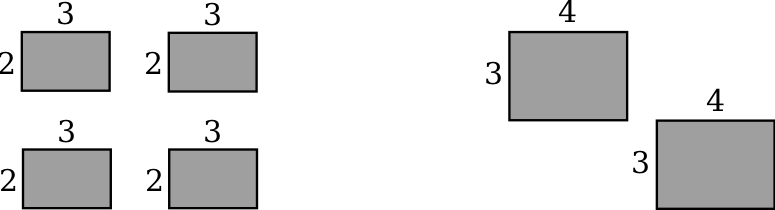
\includegraphics{assMult.png}
\end{image}
Jesse claims that these pictures represent $(2\cdot 3)\cdot 4$ and
$2\cdot (3\cdot 4)$.
\begin{enumerate}
\item Is Jesse's claim correct? Explain your reasoning.
\item Do Jesse's pictures show the associativity of multiplication? If
  so, explain why. If not, draw new pictures representing $(2\cdot
  3)\cdot 4$ and $2\cdot (3\cdot 4)$ that do show the associativity
  of multiplication.
\end{enumerate}
\end{problem} 

\begin{problem}Explain what it means for an operation $\star$ to be
  \textit{commutative}. Give some relevant and revealing examples  and non-examples.
\end{problem} 

\begin{problem}Explain what it means for an operation $\star$ to \textit{distribute}
  over another operation $\dagger$. Give some relevant and revealing
  examples and non-examples.
\end{problem} 

\begin{problem}Explain what it means for an operation $\star$ to be \textit{closed}
  on a set of numbers. Give some relevant and revealing
  examples and non-examples.
\end{problem} 

\begin{problem}Sometimes multiplication is described as \textit{repeated
  addition}. Does this explain why multiplication is commutative? If
  so give the explanation. If not, give another description of
  multiplication that does explain why it is commutative.
\end{problem} 

\begin{problem}In a warehouse you obtain $20\%$ discount but you must pay a
  $15\%$ sales tax. Which would save you more money: To have the tax
  calculated first or the discount? Explain your reasoning---be sure
  to use relevant terminology.  In particular, which property 
of which operation(s) do you use?  
\end{problem} 

\begin{problem}Money Bags Jon likes to give a tip of $20$\% when he is at
  restaurants. He does this by dividing his bill by $10$ and then
  doubling it. Explain why this works.
\end{problem} 

\begin{problem}Regular Reggie likes to give a tip of $15$\% when he is at
  restaurants. He does this by dividing his bill by $10$ and then
  adding half more to this number. Explain why this works.
\end{problem} 

\begin{problem}Wacky Wally has a strange way of giving tips when he is at
  restaurants. He does this by rounding his bill up to the nearest
  multiple of $7$ and then taking the quotient (when that new number
  is divided by $7$). Explain why this isn't as wacky as it might
  sound.
%% \begin{teachingnote}
%% The problem above is fundamentally different than the other (related)
%% problems involving tips.
%% \end{teachingnote}
\end{problem} 

\begin{problem}Cheap Carl likes to give a tip of $13\frac{1}{3}$\% when he is
  at restaurants. He does this by dividing his bill by $10$ and then
  adding one-third more to this number. Explain why this works.
\end{problem} 

\begin{problem}Reasonable Rebbecca likes to give a tip of $18$\% when she is at
  restaurants. She does this by dividing her bill by $5$ and then
  removing one-tenth of this number. Explain why this works.
\end{problem} 

\begin{problem}Can you think of and justify any other schemes for computing the
  tip?
\end{problem} 


\end{document}